

\documentclass[runningheads,a4paper]{llncs}

\usepackage{amssymb}
\setcounter{tocdepth}{3}
\usepackage{graphicx}
\usepackage{algorithm}
\usepackage{algorithmic}
\usepackage{url}

\urldef{\mailsa}\path|{kejriwal,tomas}@cs.utexas.edu|    
\newcommand{\keywords}[1]{\par\addvspace\baselineskip
\noindent\keywordname\enspace\ignorespaces#1}

\begin{document}

\mainmatter  % start of an individual contribution

% first the title is needed
\title{Unsupervised Online Wikification: A Light Approach}

% the name(s) of the author(s) follow(s) next
%
% NB: Chinese authors should write their first names(s) in front of
% their surnames. This ensures that the names appear correctly in
% the running heads and the author index.
%
\author{Mayank Kejriwal%
\and Tomas McCandless}

% the affiliations are given next; don't give your e-mail address
% unless you accept that it will be published
\institute{University of Texas at Austin\\
\mailsa}

%
% NB: a more complex sample for affiliations and the mapping to the
% corresponding authors can be found in the file "llncs.dem"
% (search for the string "\mainmatter" where a contribution starts).
% "llncs.dem" accompanies the document class "llncs.cls".
%

\toctitle{Lecture Notes in Computer Science}
\tocauthor{Authors' Instructions}
\maketitle

\begin{abstract}
Over the last decade, Wikipedia has emerged as the \emph{de facto} global knowledge base owing to its exponential growth in popularity. At the same time, there are many unstructured documents on the Web that can be \emph{enriched} by recognizing \emph{entities} within the document and linking them to specific pages in Wikipedia. Recent approaches have tackled this \emph{Entity Linking} problem by exploiting global and local feature engineering methods on Wikipedia \emph{dumps}. These approaches are supervised, in that they require training on manually provided data before they can disambiguate links to unknown entities. The problem is exacerbated by regular updates and additions to Wikipedia; hence, a dump cannot always be relied upon for \emph{online} wikification. In this paper, we present an unsupervised solution to online wikification by making judicious use of the Wikipedia API. To control complexity and bandwidth costs, we use conservative strategies with simple, but discriminative features. Experimental results on a test dataset used in a prior offline approach demonstrate that, in conjunction with the Wikipedia API, the best features can achieve over 80 percent accuracy on the online wikification task.  
\keywords{Wikification, Entity Linking, Text Enrichment}

\end{abstract}

\section{Introduction}

Wikification is the task of identifying entity \emph{mentions} in text and linking those mentions to referent Wikipedia pages \cite{wikification}. The motivations for solving such a problem effectively are numerous. Wikification has been shown to be useful in many natural language processing tasks, including text classification \cite{use1}, automatic topic indexing \cite{use3}, textbook enriching \cite{use2} and numerous other purposes \cite{kulkarni}. Although many wikification works differ in the \emph{document collection} they are attempting to wikify and also the \emph{degree}\footnote{There are Wikipedia articles for many common concepts (an extreme being the word `the'), which most approaches would not wikify. Clearly, there is a degree to which referent concepts \emph{should} be linked to Wikipedia or DBpedia.} of wikification, they share the common problem denoted \emph{Disambiguation to Wikipedia} (D2W) \cite{roth}. 

As an example of D2W, consider the simple sentence, \emph{I am attending Wimbledon this summer}. Assume that a named entity recognition (NER) \cite{ner} system has managed to detect \emph{Wimbledon} and \emph{summer} as relevant entities. These entities would then have to be correctly linked to the Wikipedia pages referenced by URIs \url{http://en.wikipedia.org/wiki/The_Championships,_Wimbledon} and \url{http://en.wikipedia.org/wiki/Summer} respectively. A closer look at this simple example presents two potential problems, assuming an off-the-shelf NER system works without error. The first is the decision of \emph{what} to disambiguate. This relates to the degree problem earlier mentioned. We could make the (subjective) argument that the entities \emph{I} and \emph{summer} do not need to be linked, and might distract a reader from the overall meaning of the text. Certainly, the user experience would not be satisfactory if every single entity is linked to some Wikipedia page. The second problem is that of \emph{semantic ambiguity}. `Wimbledon' in the example clearly refers to the prestigious tennis tournament, but Wimbledon is also a place in England. The problem exists because, for a given entity, there are many candidate Wikipedia links. 

Moreover, mappings may be many-many. 
That is, multiple surface forms refer to the same entity in the knowledge base, and a single
surface form can potentially refer to multiple entities in the knowledge base. For example,
George Bush, the entity who was president in 2003, can be referred to by `George Bush',
`George W. Bush', `Bush', or other surface forms. Similarly, the surface 
form `Kennedy'
can refer to any number of entities from the Kennedy family, including the president 
who was
assassinated. In many cases, it may not be possible, from the information provided in the input text, to produce the correct disambiguation with sufficient confidence. 
Furthermore, when performing entity linking \cite{cucerzan}, we cannot assume the knowledge base to always be complete. Potentially, there are entities that exist in the world but do 
not have corresponding entries in the knowledge base. This is one challenging difference between
entity linking and word sense disambiguation (WSD); when performing WSD, we can usually assume that the dictionary 
containing all the word senses is complete \cite{wsd}.

Finally, we note that the knowledge base we are attempting to link entities to in this paper is Wikipedia\footnote{Equivalently DBpedia or any other frequently used and accessed knowledge base that closely mirrors Wikipedia in content.}, which is constantly in a state of flux. As an example, both Wimbledon and the FIFA world cup finals will have finished just around the submission of this work. Not only will Wikipedia pages for those specific events be updated, but numerous auxiliary pages will also be updated\footnote{For example, the player who won the Wimbledon final, players who scored goals in the world cup final etc. will have their statistics and pages updated.}. It is not a stretch to imagine that such updates happen fairly regularly, though not all updates are of equal consequence. As a particular use-case for online Wikification, consider wikifying a \emph{breaking news} article. If the article is describing some unexpected event on which an article newly got created in the Wikipedia corpus, it will be accessible to the Wikipedia API\footnote{\url{http://www.mediawiki.org/wiki/API:Main_page}} sooner than it will be included in a dump, which are only created periodically. Training on a dump also mandates non-trivial steps such as curation, indexing and parsing \cite{ir}.  

To address these problems, we present a framework for unsupervised entity linking using the Wikipedia API, and basic but representative features. We note that this is a departure from recent conventional efforts that have used increasingly sophisticated (and expensive) features. We are able to narrow the gap between the supervised and unsupervised frameworks to less than 10 percent, and show improvement of over 5 percent over baseline features, using a tri-gram model and simple enhancements to baseline features. The primary goal is to present a \emph{light} system that does not require significant expertise to deploy and can operate without manual supervision. To the best of our knowledge, no work currently attempts unsupervised wikification in an online setting.

The rest of the paper is as follows. Section \ref{related} describes some related work in this area, while Section \ref{prelim} lays out some preliminaries and the problem formulation. Section \ref{system} describes the framework in some detail followed by the experimental results in Section \ref{experiments}. Section \ref{conclusion} concludes the paper.

 
\section{Related Work}\label{related}
Wikification has received increasing research attention since the paper by Bunescu and Pasca in 2006 \cite{bunescu}. They used an SVM kernel \cite{svm}, and the context around the ambiguous mention for disambiguation. However, a different model had to be trained for each mention. This limited the solution to only those ambiguous mentions on which an SVM model had already been trained. The algorithm couldn't be applied to mentions that had never been seen before (and trained on) in the training data. Mihalcae and Csomai published an influential work in 2007 that used Word Sense Disambiguation (WSD) \cite{wsd} to perform entity disambiguation and linking \cite{wikify}. Two techniques used by their proposed system, \emph{Wikify!}, included computing lexical overlap between candidate Wikipedia pages and the context of the ambiguous mention, and training a Naive Bayes classifier using ground truth from Wikipedia \emph{itself}. It is commonly observed that a Wikipedia page contains hyperlinks to other Wikipedia pages. Thus, Wikipedia pages themselves provide valuable training data, which was exploited by the supervised system in that paper.

Since 2007, increasingly sophisticated methods have been proposed to solve the problem, at the price of increasing complexity\cite{milne},\cite{cucerzan},\cite{roth},\cite{global1}. Specifically, such methods espoused moving from \emph{local} methods to \emph{global} methods. Examples of local methods are the works by Bunescu and Pasca \cite{bunescu} and the \emph{Wikify!} system \cite{wikify}. Such methods disambiguate each entity mention \emph{in isolation}. The disambiguation of the $p^{th}$ entity mention is therefore independent of the disambiguation of the $(p+1)^{th}$ entity mention. On the other hand, global methods propose to increase accuracy by performing \emph{collective} disambiguation \cite{global1}. That is, the disambiguation of an entity is now dependent on the disambiguation of other entities in the text. This leads to significant improvements if the document has \emph{thematic coherence}, which is a characteristic of many real-world documents.

Ratinov et al. formulate the problem precisely in their work on D2W \cite{roth}, and show that existing systems adhere to their formulation. Furthermore, they show that an optimal solution to the global problem is NP-hard. The differences in existing systems proposed were those involving the features they employed and also, the approximation technique they used. One important point to note is that all systems assume supervision. That is, the approximation algorithm (typically framed as a machine learning classification problem) assumes a training set, which in the spirit of the \emph{Wikify!} system, is often derived from Wikipedia itself. Although our methods and features are considerably simpler, their novelty lies in their unsupervised application and instantaneous run-time. The wikification is achieved on-the-fly. Since it is online, it can use the most recent version of Wikipedia, as opposed to previous work that relied on training data from potentially outdated dumps.   

In the Semantic Web community, an important, related research direction is automatic extraction and transformation of entities in unstructured documents, and subsequent linking to DBpedia\footnote{dbpedia.org}. A good example of such a system is LODifier \cite{lodifier}. Another effort is the work by Exner and Nugues \cite{extraction}. Although we do not use DBpedia in this paper, the principles are similar and tools like DBpedia Spotlight\footnote{\url{https://github.com/dbpedia-spotlight/dbpedia-spotlight/wiki}} can be used for online annotation in a similar manner as the Wikipedia API. In the rest of this work, we restrict attention to the Wikipedia knowledge base and API. 


\section{Preliminaries}\label{prelim}
In this section, we give a succinct description of some preliminaries to place the rest of the paper in context. For a more comprehensive discussion, we refer the reader to Ratinov et al. \cite{roth}. 
\subsection{Problem definition}
Consider an unstructured document (equivalently denoted \emph{raw text}). We assume that a set of $p$ \emph{mentions} $M=\{m_1,m_2\ldots m_p\}$ can be extracted from each such document, where each \emph{mention} is defined as a fragment of text that occurs somewhere in the body of the text. Intuitively, each mention describes an entity. In practice, note that $p$ is unknown and the extraction process is imperfect. Also assume a simplified (but still accurate) representation of the Wikipedia knowledge base as a set of $T$ \emph{links} $L=\{t_1,t_2\ldots t_T\}$. For the purposes of this section, we assume $T$ is a constant. In reality, T is a function of underlying variables like \emph{time} and \emph{language}. In the rest of the work, we assume the English language, though the techniques can be applied to other languages for which the API can be invoked. 

There are two tasks that now need to be undertaken, \emph{ranking} and \emph{linking}. Ranking assumes that some underlying system\footnote{The Wikipedia API, for example, but also offline systems previously proposed in the literature} is able to generate a set of \emph{candidate links} for a given mention $m$ (we drop the subscript for ease of exposition). Let this candidate set be $L'_m \subseteq L$. Intuitively, such a candidate set represents candidates for disambiguating the mention. The goal of ranking is to turn this set into an ordered list, based on some ranking algorithm. Since the original paper \cite{bunescu}, techniques have relied primarily on machine learning. We explicitly assume that each mention has \emph{at most} one correct candidate disambiguation. A \emph{k-correct} ranking would then place the correct candidate disambiguation (if it exists) in the top $k$. 

Linking is a \emph{binary} classification problem that takes as input a mention and a \emph{single} candidate disambiguation (usually output by the ranker) and with the help of contextual features, decides whether the candidate disambiguation is the correct one. Although linking might seem easier than ranking, it was empirically shown to be quite difficult in practice, even in the supervised setting \cite{roth}. The reason is that contextual features can be misleading with respect to \emph{nulls}. That is, it is difficult to tell when \emph{not} to link a candidate. Accuracy was often driven down by \emph{false negatives} \cite{roth}.

In this paper, we are exclusively concerned with the \emph{unsupervised linking} problem. As described subsequently, we use a conservative approach that allows us to bypass ranking the candidate links returned by the Wikipedia API. This enables us to focus our resources primarily on the more difficult problem of linking. 
\subsection{Features}
In recent state-of-the-art systems, ranking and linking make use of both global and local features. For ranking, assume that we have a set $L'_m$ of candidate links for all mentions $m \in M$. The ranking of each list can either occur independently of each other (local) or be dependent on each other (global). The global optimization was shown to be NP-hard \cite{roth}. For linking, an analogous procedure applies. Clearly, global methods are expensive but have higher accuracy if we assume the documents to have thematic coherence. This assumption is problematic if the document has variety in its descriptions. We explore the role of different features empirically in Section \ref{experiments}.

\section{System}\label{system}

The overall system schematic is shown in Figure \ref{fig0}. The only input to the system is the unstructured document or the raw text. An off-the-shelf Named Entity Recognizer (NER) first extracts the set of mentions from the raw text. These mentions are sent on to the Wikipedia API. In this paper, we use the Stanford NER \cite{stanford}, which was also the NER used by the authors of the state-of-the-art GLOW system \cite{roth}. The NER is available freely\footnote{\url{http://nlp.stanford.edu/software/CRF-NER.shtml}}. In the subsequent sections, we describe the remaining sub-modules that were used in the framework. 

\begin{figure}
\centering
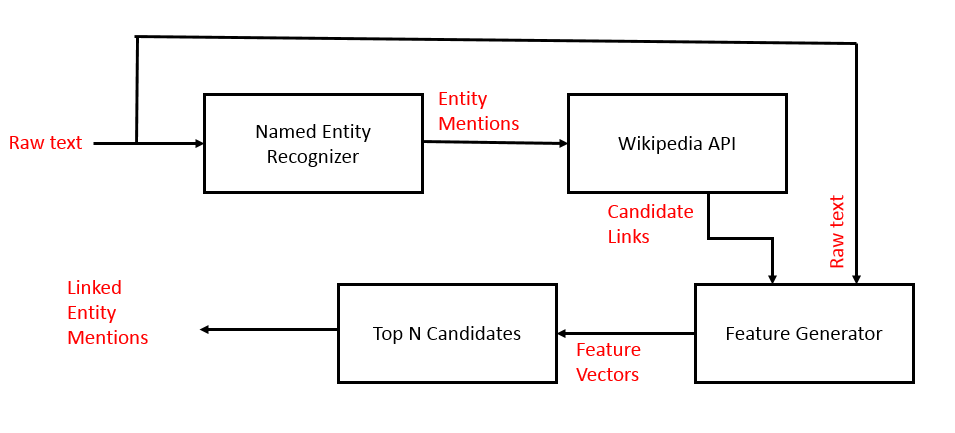
\includegraphics[height=5cm, width=12.5cm]{schematic}
\caption{The overall schematic of the proposed online wikifier.}
\label{fig0}
\end{figure}

\subsection{Wikipedia API}
Given a list of entity mentions that is output by the NER submodule, we rely on the 
Wikipedia API to extract (and return, via a REST protocol) the raw text of the candidate Wikipedia pages. Some 
named entities are ambiguous in the sense that they could refer to one of many different
Wikipedia articles. For example, the named entity `labour party' could refer to
`Social Democratic and Labour Party',
`Socialist Labor Party of America', or any number of other labour parties from many
different countries. For our particular application we are more focused on accuracy 
than coverage. Thus, when multiple candidates are returned,
we choose not to perform any linking. This conservative strategy leads to several links getting missed empirically, but the number is not as great as we might assume. Empirically, the majority of relevant mentions in the test suite (and in other documents we analyzed) had one candidate. We give specific statistics in Section \ref{experiments}. 

In its defense, the conservative decision was found to lead to fast wikification in practice, since less raw text has to be delivered over the Internet. Given that Wikipedia pages are quite long, adopting a liberal strategy\footnote{Getting all candidate links, with corresponding raw texts.} often led to payloads of a few megabytes getting returned \emph{per} page. Generating features and processing these pages (see the next section) was not instantaneous for such payloads, which is at odds with its online, real-time specification. The other usual assumptions for such payloads are, of course, sufficiently reliable REST calls to the API, as well as fast data connection. The conservative strategy minimizes the scope of these assumptions. 

Another motivation for the conservative strategy is that we empirically observed a significant slowdown when invoking the API too many times. Given that the system is intended for public deployment\footnote{The system is light enough that we are currently investigating a mobile app version for it, together with a browser extension. We believe that it is feasible to wikify and render annotated HTML pages as the user requests those pages, even on a cellular connection in a mobile browser.}, this is not a desirable trait. To improve recall, more sophisticated measures would have to be considered, but we leave for future work to determine the best way to achieve the performance improvement without burdening the online component. One such approach might be to set a threshold, such that mentions with more candidate links than the threshold number would get rejected. The conservative strategy is simply a special case of the former approach, with the threshold set to 1.  

Once obtained, the candidate pages, and also the original raw text, are input to the feature generator described in the next section. Our interface to the Wikipedia API is implemented in Python, and included with the other codebase and test suite on the companion page\footnote{\url{https://sites.google.com/a/utexas.edu/mayank-kejriwal/online-wikification}}.
\subsection{Feature Generator}
Features form the backbone of our system. A literature survey of existing wikifiers show that the primary difference between them lies in the complexity and expressivity of their features. Online wikification demands features that are simple yet representative. Towards this end, we devised three simple features to be used in conjunction with any n-gram model (including a bag of words model). The first of these is TF-IDF. The IDF is computed over the set of Wikipedia pages returned for the mentions in a raw text. Thus, a different IDF (an `on the fly' IDF) would be computed for each raw text document. We also experiment with TF and stop-words, that is, removing common stop-words before computing normalized TF vectors. Finally, we combined stop-words and IDF with TF. Note that the feature generator outputs a feature vector for each candidate Wikipedia page corresponding to a mention in the raw text and also outputs a feature vector for the raw text itself. The second (non-IDF) feature can be computed in a streaming fashion, but the other two require the first module to have finished retrieving all the candidates before calculating the feature vectors. We also assume that a small list of stop-words are provided to the system a priori. Such lists are quite extensively available\footnote{We used the one provided by \url{http://ir.dcs.gla.ac.uk/resources/linguistic_utils/stop_words} in our implementation.}. 
\subsection{Top N Candidates}
The goal of this module is to take the Wikipedia feature vectors and the raw text feature vector extracted by the feature generator  together with an additional user-provided input, N. Each Wikipedia feature vector is \emph{scored} by taking its dot product with the raw text feature vector. The top N Wikipedia vectors are marked as \emph{correct} and the corresponding mentions are linked to these Wikipedia pages. We experimentally show how accuracy varies with N in Section \ref{experiments}. 

Again, a threshold and weights can be specified instead of taking a simple dot product, but determining these would require training examples. Empirically, the hope is that by choosing a moderately small N, only the most important concepts in the page are wikified, and with high accuracy. We evaluate the success of these conservative design decisions in Section \ref{experiments}.




\section{Experiments}\label{experiments}

In this section, the dataset is first described, followed by the methodology. This is followed by some results and a discussion of those results. 
\subsection{Dataset}

We used the \emph{Wiki} test set first developed by the authors of GLOW \cite{roth}. They made the dataset available on their companion project website\footnote{\url{http://cogcomp.cs.illinois.edu/data}}. The Wiki data came with training data and test data and were extracted from `difficult'\footnote{As described by the GLOW authors.} Wikipedia paragraphs (baseline features in GLOW yield at least a 10 percent error rate on these extracted paragraphs). The training data was much larger than the test data. In their work, Ratinov et al. first trained a system employing both global and local features using the training data, and then evaluated both a ranker and linker on the test data. 

Since we are only evaluating \emph{unsupervised} linking, we neglected the training data completely and evaluated the system on the test data. This data consists of 40 documents with a total of 839 mentions (extracted by Stanford NER) between them. Some of these were \emph{nulls} (that is, had no corresponding Wikipedia page according to the provided ground truth) and for others, the Wikipedia API returned multiple candidates (and that were hence ignored). In total, there were 724 mentions for which the API returned a single link\footnote{This also demonstrates that the recall of the conservative strategy is not as low as we might expect.}. Some of these returned links were `wrong' in that they corresponded to a null in the ground truth or a \emph{different} Wikipedia page than what the API returned. On average, we found about 78 percent of the returned links to be correct. Thus, a naive approach that would randomly sample N links (used as one of our baselines) would, on average, achieve this precision.   
\subsection{Methodology}
We experimented with each of the three features as well as their combinations using three language models: bag of words, bi-grams and tri-grams. For each model, two sets of experiments were conducted. Both experiments use $N$ as the independent variable, and for each document, rank the top N scoring (where the score is the dot product of the feature vectors) candidate links as correct. Accuracy is measured against N. For example, if all N chosen links are correct, the accuracy is 100 percent. Although N does not technically represent \emph{recall}, it is somewhat analogous. Note however that since we have multiple documents, there are two typical ways to calculate accuracy for a given value of N when the algorithm is run on \emph{all} documents. The first, which we call the \emph{surface forms accuracy}, is to compute the accuracy across the full set of mentions in the entire corpus. There is no averaging across documents. The second is to compute the accuracy for each document individually, and to then average accuracies across documents, with each document getting equal weight (\emph{documents accuracy}). As a simple example of the difference, suppose there are two documents with 20 mentions in the first document and 40 mentions in the second. Suppose, on average, that the accuracy on the first document is 80 percent, and on the second is 75 percent. The documents accuracy would then simply be 77.5 percent. However, the surface forms accuracy would be $(.75*40+.80*20)/60=76.667$ percent. We show the results for both forms of averaging in the experiments.
Recall that one of the features proposed is that of stop-words removal. We used two baselines: random selection of N candidates and normalized TF. By supplementing normalized TF with IDF, stop-words removal or both, we measure the enhancement in performance for all the models.
\subsection{Results and Discussion}
The first interesting trend observed in all the figures is that a standard tradeoff is not observed, where accuracy would decline with increasing N. Instead, the figures yield a flat curve of about 78 percent for the surface forms accuracy and 77 percent for the documents accuracy. In general, absolute differences aside, the surface forms accuracy and documents accuracy curves were found to mirror each other closely (with only about one percent difference in absolute numbers) so we refer to a single curve in the following discussion (surface forms). The value of N at which accuracy peaks is between 15 and 20 for all the figures. 

More surprisingly, the TF baseline actually performs worse than the random baseline till this peak value, after which it usually shows slight improvement, before leveling off with the other curves. Note also that the combination of features (TF, IDF and stop-words) works best, but except on the bigrams model, the other features actually show better performance on \emph{lower} values of N. The best performance for N between 2 and 5 was demonstrated by TF and IDF on the trigrams model. Over that range, it briefly outperforms the combined three features of TF, IDF and stop-words.

It is interesting to compare the unsupervised performance with the supervised performance using a much more sophisticated method and features than what we used (in the original GLOW paper) \cite{roth}. Using a trained linker, the authors were able to achieve about a 92 percent accuracy . As mentioned earlier, the training data was much larger than the test data, yielding high levels of supervision. The ranker accuracy was also assumed to be perfect when evaluating the linker in the original paper \cite{roth}. Thus, the only task addressed was determining the `nulls' in the ground truth. On the other hand, we had to rely on the Wikipedia API for our `ranker candidate'. Some of these were wrong. In this sense, the unsupervised linker problem is harder, since we have to determine both nulls (mentions that don't correspond to a Wikipedia page at all in the gold standard) as well as mentions for which wrong links were returned by the API. Although the 10 percent difference is considerable, we believe it can be narrowed by including other inexpensive features and heuristics.  An encouraging result is that, by using a tri-gram model with some intuitive enhancements, an accuracy of over 83 percent was achieved over a small range for N. 

\begin{figure}
\centering
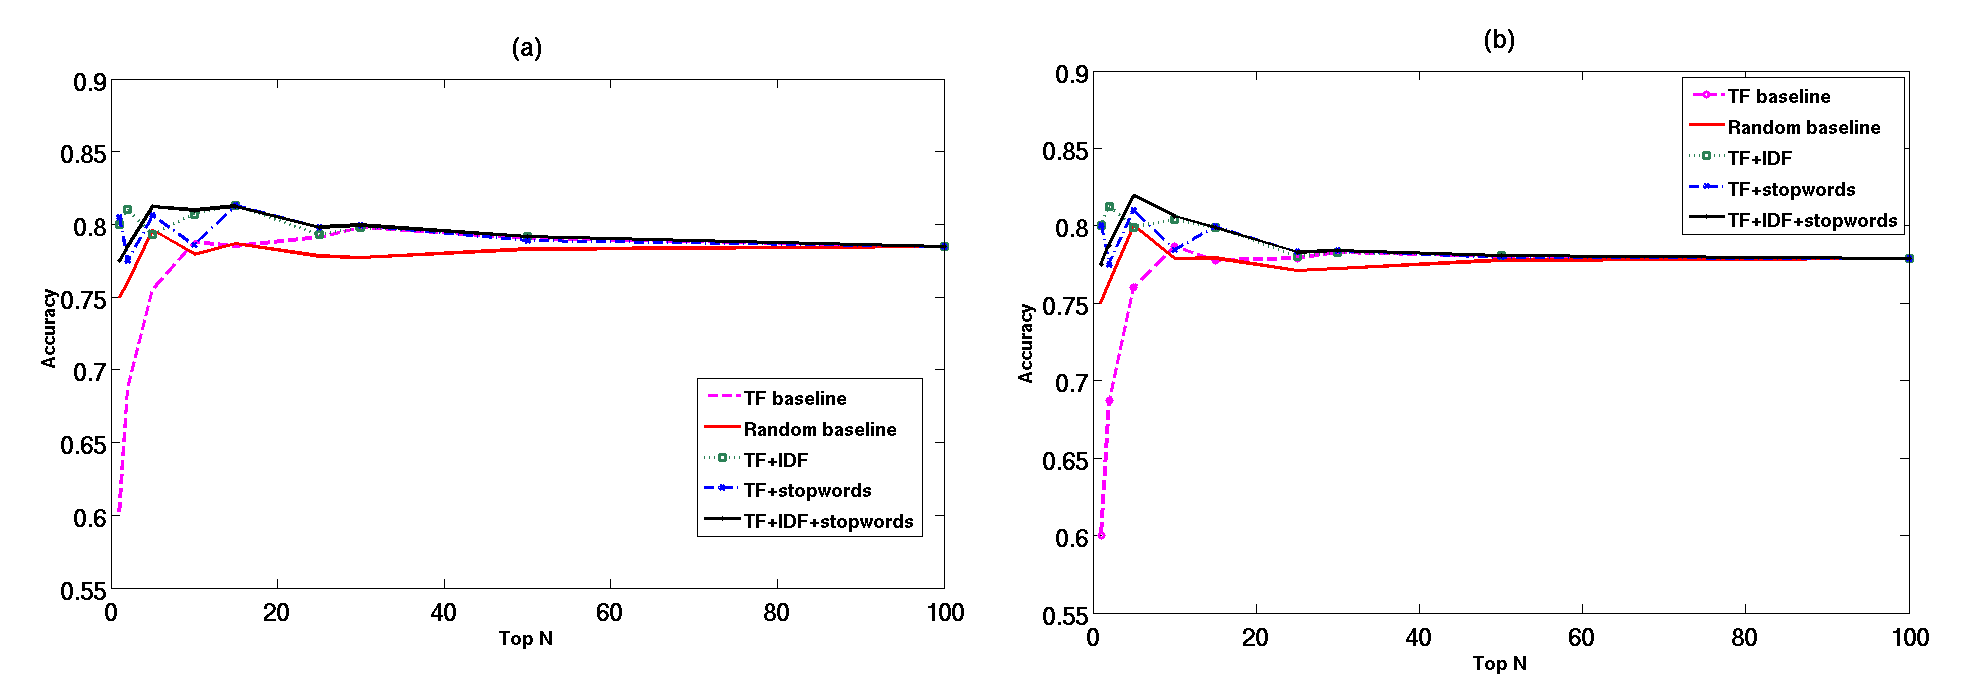
\includegraphics[height=5cm, width=12.5cm]{normal}
\caption{Results of the procedure when no n-gram features are employed. (a) represents surface forms accuracy and (b) shows documents accuracy}
\label{fig1}
\end{figure}
\begin{figure}
\centering
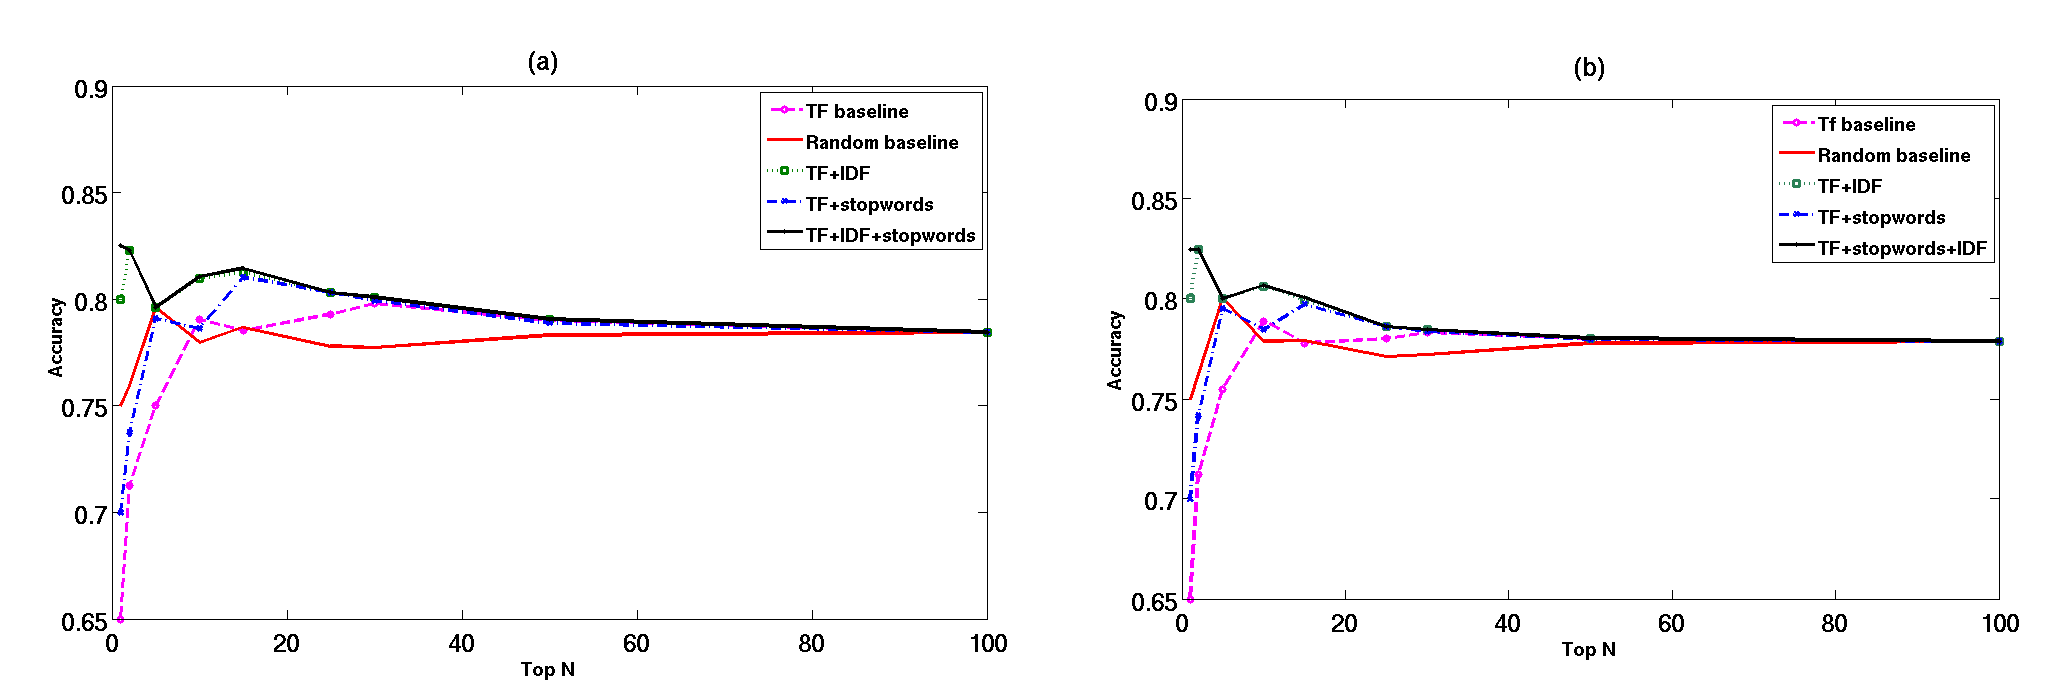
\includegraphics[height=5cm, width=12.5cm]{bigrams}
\caption{Results of the procedure when TF includes bi-gram features. (a) represents surface forms accuracy and (b) shows documents accuracy}
\label{fig1}
\end{figure}
\begin{figure}
\centering
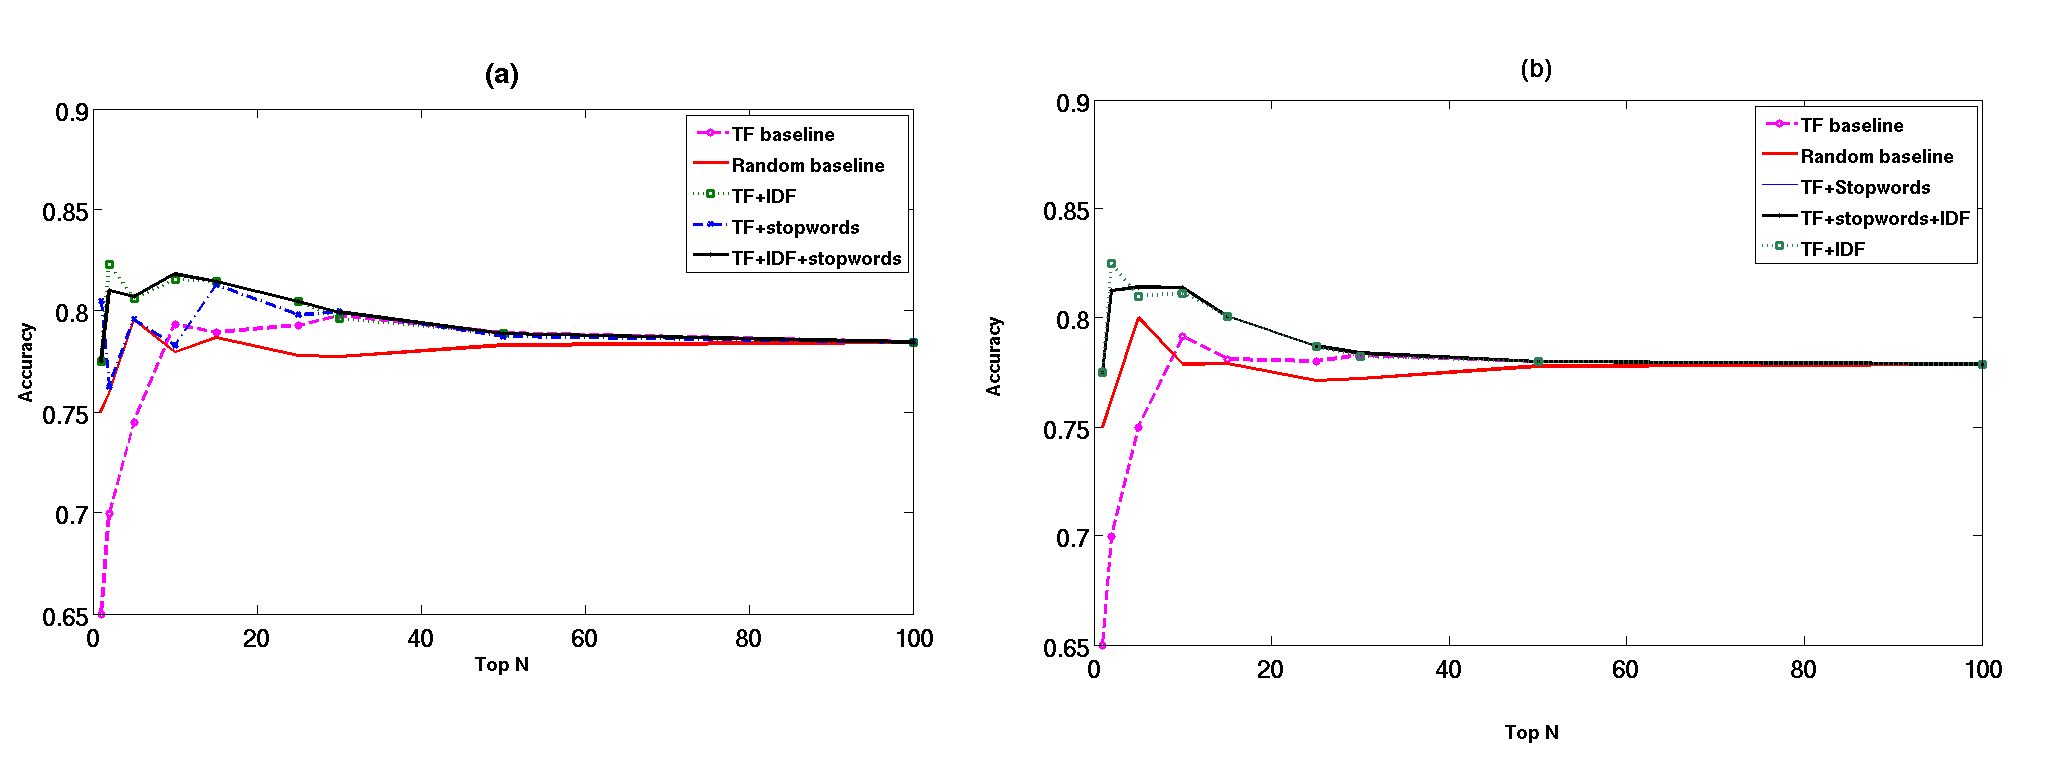
\includegraphics[height=5cm, width=12.5cm]{trigrams}
\caption{Results of the procedure when TF includes tri-gram features. (a) represents surface forms accuracy and (b) shows documents accuracy}
\label{fig1}
\end{figure}

\section{Conclusion and Future Work}\label{conclusion}
In this paper, we presented a practical solution to unsupervised entity linking using the Wikipedia API. Using bi-gram and tri-gram models, together with enhancements to basic features like TF, we achieved a 5 percent performance boost on baseline features and narrowed the gap between supervised and unsupervised linker accuracy to less than 10 percent. The key advantages of the proposed system is that it is light, has low bandwidth and computational costs, relies on tools that are freely available and most importantly, can be extended to other knowledge bases that offer similar access points. We expect the system to be particularly amenable to mobile deployment; for example, as a mobile Semantic Web app.

Future work will investigate the challenges of this deployment more closely, along with attempting to narrow the observed supervised-unsupervised performance gap through better features. We will also carry out user studies to determine both the values of N and the minimum accuracy expected for a satisfactory user experience.    


\bibliography{typeinst}
\bibliographystyle{abbrv}
\end{document}
